%
% Template for DCS course projects
%
\documentclass[a4paper,11pt,oneside]{book}
\usepackage[latin1]{inputenc}
\usepackage[english]{babel}
\usepackage{amsfonts}
\usepackage{amsmath}
\usepackage{amssymb,amsmath,color}
\usepackage{cite}
\usepackage{graphicx}
\usepackage{float}
\usepackage{algorithm}
\usepackage[noend]{algpseudocode}

\makeatletter
\def\BState{\State\hskip-\ALG@thistlm}
\makeatother

\begin{document}
	\pagestyle{myheadings}
	
	%%%%%%%%%%% Cover %%%%%%%%%%%
	\thispagestyle{empty}                                                 
	\begin{center}                                                            
		\vspace{5mm}
		{\LARGE UNIVERSIT\`A DI BOLOGNA} \\                       
		\vspace{5mm}
	\end{center}
	\begin{center}
		
\includegraphics[scale=.27]{figs/logo_unibo}
	\end{center}
	\begin{center}
		\vspace{5mm}
		{\LARGE School of Engineering} \\
		\vspace{3mm}
		{\Large Master Degree in Automation Engineering} \\
		\vspace{20mm}
		{\LARGE Distributed Control Systems} \\
		\vspace{5mm}{\Large\textbf{COVERAGE CONTROL FOR COOPERATIVE MULTI-ROBOT NETWORKS}}                  
		\vspace{15mm}
	\end{center}
	\begin{flushleft}                                                                              
		{\large Professor: \textbf{\@ Giuseppe Notarstefano}} \\        
		\vspace{13mm}
	\end{flushleft}
	\begin{flushright}
		{\large Students:\\
			\textbf{Donato Brusamento\\
				Mattia Micozzi\\
				Guido Carnevale\\
				Lorenzo Draghetti}}\\
	\end{flushright}        %capoverso allineato a destra
	\begin{center}
		\vfill
		{\large Academic year \@2018/2019} \\
	\end{center}
	
	
	\newpage
	\thispagestyle{empty}
	
	%%%%%% ABSTRACT %%%%%%%%%%
	
	
	\begin{center}
		\chapter*{}
		\thispagestyle{empty}
		{\Huge \textbf{Abstract}}\\
		\vspace{15mm}
	\end{center}
	The aim of the project hereby presented was to transpose the algorithms described in the research paper\cite{K1} into a proper Matlab environment suitable for simulation and results analysis.\\\\
	
	The aforementioned algorithms has been simplified in order to adapt to both an offline, sequential approach (from now on called \textbf{offline},or \textbf{centralized}) and to a parallel (single machine), asynchronous one (from now on called \textbf{online},or \textbf{distributed}).\\
	In both approaches, the simulation implements a simple proportional closed loop control, but while in the former it is all done inside a centralized \textit{for loop}, in which informations about each agent is readily available to all others, in the latter we tried to be more faithful to the original formulation, in which every agents has to exchange with other agents informations about each other's positions in a timely manner, while being "deaf" (to a certain extent) in-between successive communications.\\\\
	
	To achieve all of this we've made use of Matlab's \textit{Parallel Computing Toolbox} to simulate the independent agents as communicating threads.\\
	In the distributed version of the simulation we also implemented a visual comparison between the two approaches so to show how they bring slightly different results.
	
	
	%%%%%%%%%%%%%%%%%%%%%%%%%%%
	
	\tableofcontents \thispagestyle{empty}
	\listoffigures\thispagestyle{empty}
	
	%%%%%% INTRODUZIONE %%%%%%%%%%
	\chapter*{Introduction}
	\addcontentsline{toc}{chapter}{Introduction}
	A mobile wireless sensor network (MWSN) can be defined as a wireless sensor network (WSN) in which the sensor nodes are mobile. For example the nodes can be wheeled robots scattered in a given area.\\\\
	MWSNs are an emerging field of research in contrast to their well-established predecessor. They are way more flexible than static sensor networks as they can be deployed in any scenario and deal with rapid topology changes due to node failures or new added sensors. In general each node consists of a radio transceiver, a microcontroller powered by a battery and one or more sensors to detect certain properties of the environment.~\cite{K2}\\ 
	Typical applications of this kind of network are environment monitoring, surveillance, search and recovery operation, exploration.\\
	A problem that can arise in this context is the optimization of coverage of a given area knowing the density distribution function, defined on that area, of a given property we would like to measure. The objective of this project was to implement a distributed and asynchronous algorithm to solve this problem, following the method proposed in the research paper \cite{K1}.\\\\
	The considered framework, as suggested by the aforementioned paper, is the following: n mobile sensor-robots modelled as simple integrators strewn on an area given by a convex polytope defined in $\mathbb{R}^2$; on this area a 2-dimensional distribution $\phi:Q\rightarrow \mathbb{R}_+$ is defined to represent the density of the feature that nodes have to measure.\\ Each node has sensing (can locate the other nodes positions) and/or communication capabilities.  \\
	
	Conceptually this algorithm runs iteratively 2 subroutines: one, called "Adjust-sensing radius algorithm", to compute the Voronoi cell of each sensor, and another one, called "Monitoring algorithm" to check if the computation of the Voronoi cell has to be updated because of significant changes in the network (variation of nodes positions, node failures,...).\\\\\\\\
	
	
	
	We implemented this procedure in Matlab in 2 ways:
	\begin{enumerate}
		\item in a centralized sequential way
		\item in a distributed parallel fashion, reading and writing files (stored in a master server) to realize communication among nodes.
	\end{enumerate}
	These two implementations and the differences between them are well-explained and analysed in this report\\
	In particular, the first chapter regards the problem set-up and description of proposed solutions; the second chapter contains the analysis of obtained results.\\
	
	
	\section*{Motivations}
	The algorithms and simulations have been implemented in Matlab because of its (relatively speaking) simplicity and useful add-ons.\\
	In particular, thanks to the graphical tools readily made available we could also create a real time results visualization to accompany the simulations, which is well suited to analyse the behaviour of both algorithm, compare them, and easily fix or add missing features.
	
	
	\section*{Contributions}
	We believe that, thanks to this project, we created a starting point for building and implementing on real MWSN the proposed control algorithms; while further steps have to be taken in the direction of optimizing the code for embedded platforms (and simulations as well), the main idea of the paper used as a guideline, and its efficiency, have been demonstrated through our framework.
	
	%\section*{Organization}
	%%%%%%%%%%%%%%%%%%%%%%%%%%%%%%%
	
	%%%%%%%%% CAPITOLO  %%%%%%%%%%%%%%%%
	\chapter{Problem set-up and solutions}
	First-chapter for problem set-up and description of the implemented solution. 
	
	\section{Setup}
	\subsection {Theoretical notions}
	
	The algorithm proposed by the main paper is \textbf{Lloyd's gradient descent}, which guarantees the convergence to an optimal solution intuitively given by the trade-off between each node's coverage (position) and relative degradation of sensing capabilities.\\
	A main point to be considered is that this solution makes use of the concept of Voronoi partitions.\\
	Given a subspace $S$ in $\mathbb{R}^N$ (typically a plane) and a set of n points $P=\{p_1,...,p_n\}$ belonging to this subspace we call Voronoi partition a partition such that there is an associated region for each point and this region consists of all points closer to that point than any other point. We call these regions Voronoi Cells.\\
	Let's see an example of Voronoi Partition of a plane:\\
	
	\begin{figure}[hb]
		
		\centering
		
		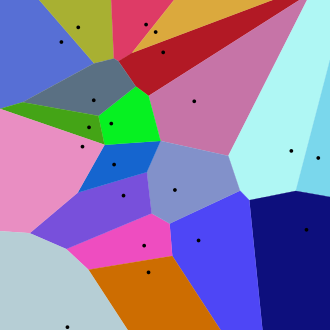
\includegraphics[scale=0.33]{figs/VoronoiPartition.png}
		\caption{Voronoi Cells of 20 points on a plane}\label{fig:Voronoi Partition.png}	
	\end{figure}
	

	Considering a convex polytope $Q$ in $\mathbb{R}^N$ and n sensors, for the sensor positions $P=\{p_1,...,p_n\}$ the optimal partition of $Q$ is the Voronoi partition  $V(P)=\{V_1,...,V_n\}$, where $V_i$ is the Voronoi cell of the i-th sensor: $$V_i=\{q\in Q|\> \|q-p_i\|\le\|q-p_j\|, \forall j\not= i\}$$\\
	Intuitively speaking, each $V_i$ represents the region of space in which the respective sensor i is performing its task.\\
	
	
	Citation \cite{K1}\\
	
	Because of noise and loss of resolution we assume also that the sensing quality of a sensor placed at $p_i$ wrt a point $q$ decreases as much the distance between $p_1$ and $q$ is large. Then once we have computed the Voronoi Partition we have also to find for each Voronoi Cell the point in which the sensing degradation is minimized in order to move the sensor in this point.\\
	Obviously this motion modifies the situation and may change the Voronoi Partition. As in the paper we have modeled the sensing degradation as the squared distance between the sensor location and the considered point. Under this assumption we have that for each Voronoi Cell the point in which the sensing degradation is minimized is the so called generalized centroid $C_v$ of the Voronoi Cell namely the center of mass (generalized mass $M_v$) that we find considering the distribution density function of the variable that we want to measure as a mass density function $p$.\\
	
	                $M_v$=$\int_{V} p(q)\, dq$  \\\\ 
	    
	                $C_v$=$\frac{1}{M_v} \int_{V} q p(q)\, dq$  \\\\
	
	The adopted alogrtihm \textbf{Lloyd's gradient descent} guarantees to reach a global convergence under the given assumptions.   
	
	\subsection{Adopted assumptions}
	
	Although the code was implemented with the objective in mind of staying as much faithful to the paper as possible, some assumptions had to be made in order to work with the simulations running on a single machine, especially considering that some pieces of code (e.g. the computation of Voronoi cells) tend to slow them down quite a bit, and should then be optimized during further developments.\\ %(with a deeper proficiency of coding and mathematical skills that are unfortunately not in possession of anyone of us at the time of this writing).\\
	
	In particular, with respect to the "ideal" version of the algorithm proposed in the paper\cite{K1}, the assumptions made are
	
	\begin{enumerate}
		\item The \textit{sensing} of other agents is not implemented by a specific communication protocol; in the distribution version case, text files were written and read in a similar fashion to \textit{POSIX pipes}, and the only reason preventing an immediate sensing is the lock put to files during mutual r/w.\\This, as a side effects, also "forces" the lack of synchronism between threads.
		
		\item The \textit{timing}, as in the scheduling of different subroutines like monitoring and sensing, is not implemented, as it would require real platforms with only few unique threads running so to not introduce large discrepancies in convergence speeds.\\
		This is not only due to (rather severe) constraints of horsepower available on the used machines, but also to the lack of ready to use, POSIX-like scheduling primitives in Matlab's \textit{Parallel Computing Toolbox}.\\
		On top of that, while this would definitely be an issue in the real world implementation of the algorithm, for the purpose of this project (i.e. demonstration and simulation of the algorithm and creation of essential tools for its correct implementation), the proposed version suffices in its goals, and the following point explains the trade-off that was made in accordance with the professor's directions.
		
		\item For the same reason, while the correct calculation of neighbours weights is implemented and also displayed in the Offline algorithm, in the Distributed version agents do not wait for \textit{events} in order to change control, but rather they first reach the last computed region's centroid, and only then they sense others' position to update their own cell and reference centroid.\\
		However, should the need arise, the primitives and functions aiding in the event generation are already available in Ver. A of the code, as mentioned.
		
		
	\end{enumerate}
	
	
	
	
	\section{Inner Workings}
	\subsection{Offline algorithm (A)}
	
	As said before, in this project two ways to reach the final goal have been followed: the \textbf{centralized} algorithm, namely the one which exploits the fact that each position of each agent is known by the others, and the control law is applied in a \textit{sequential} manner, is developed in this section.\\
The fig.~\ref{fig:algorithmA.png} allows a more comprehensive approach to the explanation of this algorithm.\\
The initialization phase lets the user to generate the workspace randomly, or to upload a given benchmark to work with. \\
If the former choice is made, a set of functions will be called:
 \begin{itemize}
		\item \textit{buildArea}: it creates a convex area, namely a polygon with a given number of vertices placed in a given range of the plane;
		\item \textit{generateAgents}: it places a fixed number of agents in the already built area, positioning them randomly;
		\item \textit{genPolyGrid}: it turns the plane individuated by the area of the polygon into a discrete grid of points, in order to build the probability distribution function.  
		\item \textit{gaussianDistr2d}: it generates a 2-dimensional Gaussian distribution function that represents the distribution of the information to be acquired. 
\end {itemize}
The latter choice allows to take all of this material from an external file.\\

Once all the benchmark features are defined, the algorithm makes a first computation of the Voronoi cells, analyzing and classifying the neighbours of each agent, and estimating the \textit{centroid} of each cell, weighted with respect to the density. To this purpose, some complex functions have been developed, that will be discussed further:
\begin{itemize}
	\item \textit{calculateCell};
	\item \textit{sliceCell};
	\item \textit{genMCgauss}.
\end{itemize}
Thus, after the first partition of the main area, the control parameters are defined, and the control action can start.\\
Since the project assumptions state that each agent must be considered as a single-integrator, the control consists only in a proportional action aimed to fill the gap between the agent position and the centroid of its Voronoi cell. The sequential fashion is implemented by means of a \textit{for loop}, that lets the agents move one by one, toward its own Voronoi centroid.\\
In each iteration, actually, the single agent doesn't reach necessarily the goal (namely, the centroid), and at the beginning of the next iteration, it computes another time its Voronoi cell, updating the centroid if some changes happened in the neighbourhood.\\
In this way, each agent approaches constantly a reference that is moving in time, because actually at each iteration the centroid is updated. \\
Finally, the algorithm stops when every agents has reached a distance from its cell centroid lower than a given threshold.\\	
	\begin{figure}
		
		\centering
		
		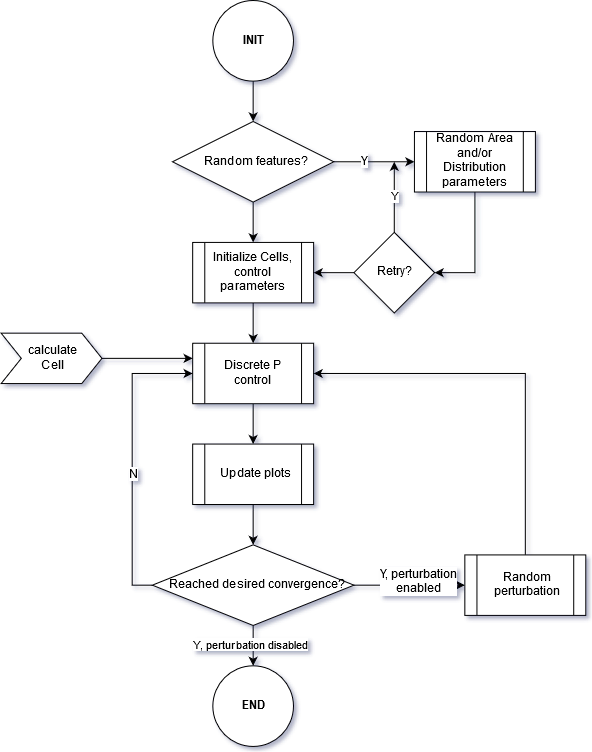
\includegraphics[scale=0.63]{figs/algorithmA.png}
		
		%%%%%%%%%%%%%%%%%%%%%%%%%%%%%%%%%%%%%%%%%inserisce la legenda ed etichetta
		%   la figura con \label{fig:prima}
		\caption{Algorithm A flow}\label{fig:algorithmA.png}
		
	\end{figure}
	
	\subsection{Online algorithm (B)}
	
	\begin{figure}
		
		\centering
		
		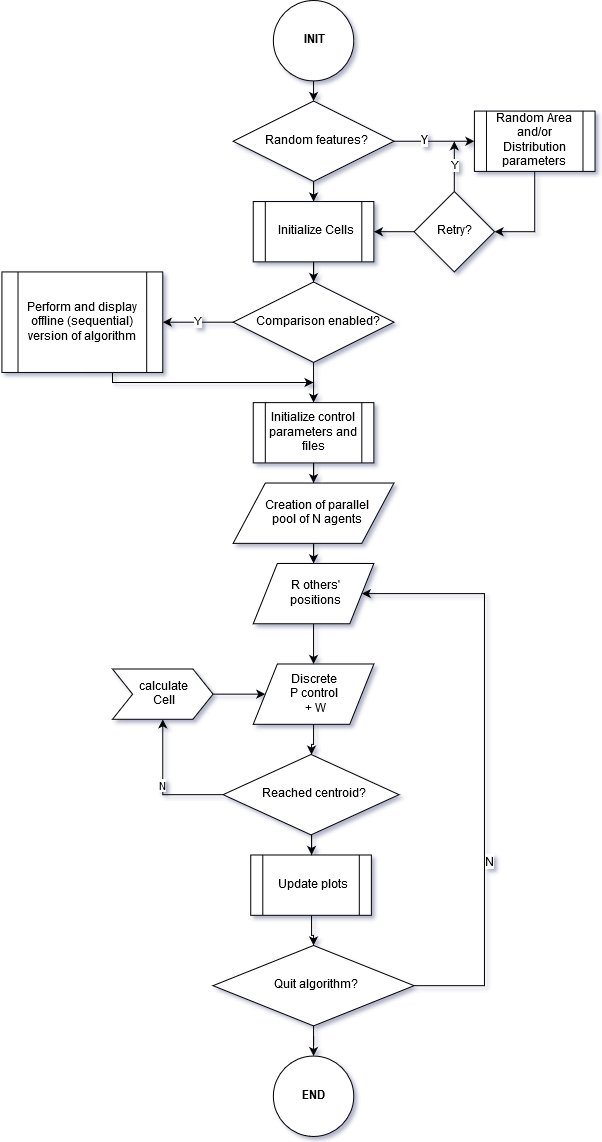
\includegraphics[scale=0.55]{figs/algorithmB.png}
		
		%%%%%%%%%%%%%%%%%%%%%%%%%%%%%%%%%%%%%%%%%inserisce la legenda ed etichetta
		%   la figura con \label{fig:prima}
		\caption{Algorithm B flow}\label{fig:algorithmB.png}
		
	\end{figure}
	
	\subsection{Utils}
	\subsubsection{calculateCell}
	This function is the one that implements the \textit{Adjust Sensing Radius Algorithm} presented in \cite{K1}.\\
	 Its purpose is to compute the Voronoi cell of each agent, modifying the sensing radius in order to converge to a unique and correct solution.\\
	 The function is slightly different in the two versions of the project, in the offline version (\textit{ver. A}), as already mentioned, the function provides also the calculations of the neighbours weights; feature not present in the online version.
	 As input it needs:
	 \begin{itemize}
	 	\item the actual position of the agent;
		\item the initial radius (arbitrarily small);
		\item the total working area;
		\item (\textit{only for the offline version}) the position and the status of all the agents;
	\end{itemize}
The algorithm of the function can be summarised in the table below:
	\begin{algorithm}
\caption{calculateCell}\label{euclid}
\begin{algorithmic}[1]
\State intersect the initial radius with the allowable area
\BState \emph{loop}:
\If {any other agent \emph{j} found} 
\State store \textit{ID} and \emph{distance} from the agent in exam inside a \emph{table}
\EndIf
\State sort the table by increasing distance from the agent
\If {the table is not empty}
\State run \emph{sliceCell} for each agent in the table
\EndIf
\State compute the new estimated cell
\If {the radius is smaller than twice the distance between the agent and the furthest vertices of the cell}
\State double the radius
\State \textbf{goto} \emph{loop}
\Else  
\State save the actual radius
\State save the weights of the neighbours
\State save the final cell
\EndIf
\State \textbf{close}
\end{algorithmic}
\end{algorithm}	

	\subsubsection{sliceCell}
	\subsubsection{genMCGauss}
	
	
	%%%%%%%%% CHAPTER  %%%%%%%%%%%%%%%%
	\chapter{Results analysis}
	
	\section{Prerequisites}
	%put necessary toolboxes and FEX files here
	For the correct functioning of the simulations, the following Matlab Toolboxes and FEX files should be installed:
	
	\begin{itemize}
		\item Parallel Computing Toolbox
		\item Mapping Toolbox
		\item labelpoints, by Adam Danz
		\item Fast and Robust Curve Intersections, by Douglas Schwarz
	\end{itemize}
	
	\section{Simulation benchmarks}
	
	In both approaches, several parameters can be adjusted that affects precision (and conversely, speed of simulations), namely:
	
	\begin{itemize}
		\item number of agents;
		\item query points density for distribution computation;
		\item proportional gain of the control;
		\item convergence threshold;
		\item etc.
	\end{itemize}
	
	In addition to that, the generation of the area to cover, of the agents and of the distribution can be set to randomly generate at each start of simulation (see fig.~\ref{fig:randomAgents.png}, fig.~\ref{fig:gaussianDistrib.png}).
	
	\begin{figure}	
		\centering	
		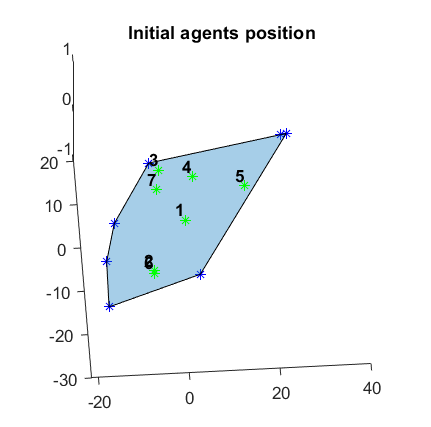
\includegraphics[scale=0.7]{figs/randomAgents.png}
		\caption{Random agents spawning}\label{fig:randomAgents.png}	
	\end{figure}
	
	\begin{figure}	
		\centering	
		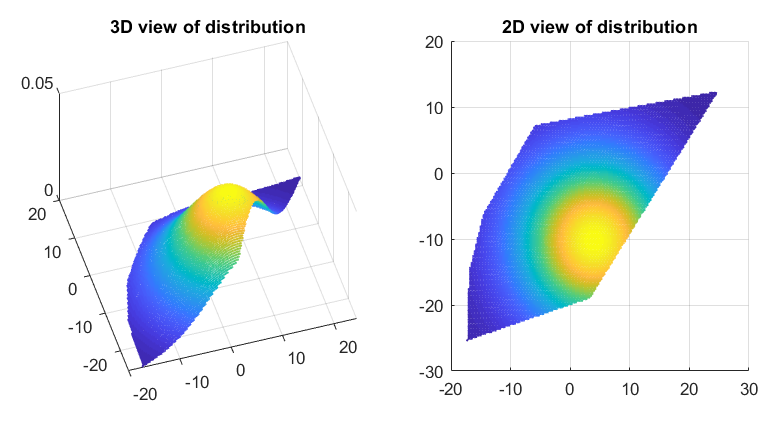
\includegraphics[scale=0.7]{figs/gaussianDistrib.png}
		\caption{Random 2D normal distribution}\label{fig:gaussianDistrib.png}	
	\end{figure}
	
	\section{Offline algorithm (A)}
	
	The simulation converges with a good speed with few agents and with a reasonable one with more (see fig.~\ref{fig:convergenceResultsA.png}, fig.~\ref{fig:20convergenceResultsA.png}); we can speculate that considering the typical speed of mobile robots the speed of every step is well suited.\\\\
	As for correctness, the only issues encountered up to now is with very few agents (4-5) and a very large area (e.g. 10000 sq. unit), for which the cells tend to not be correct, because of the way "Fast and Robust Curve Intersections" works, i.e. by intersecting bounding boxes between the two desired geometrical entities.\\
	Since the agents may be scattered around this large area, the rate of increase of the radius (that is, 2x at each successive step) bring the algorithm to find the bounding box of the radius to completely encompass the area to cover, thus not finding intersections at all; we believe that either a different increase rate of the radius, or better yet, a more efficient way to compute the Voronoi Cell may solve the issue.
	
	
	\begin{figure}	
		\centering	
		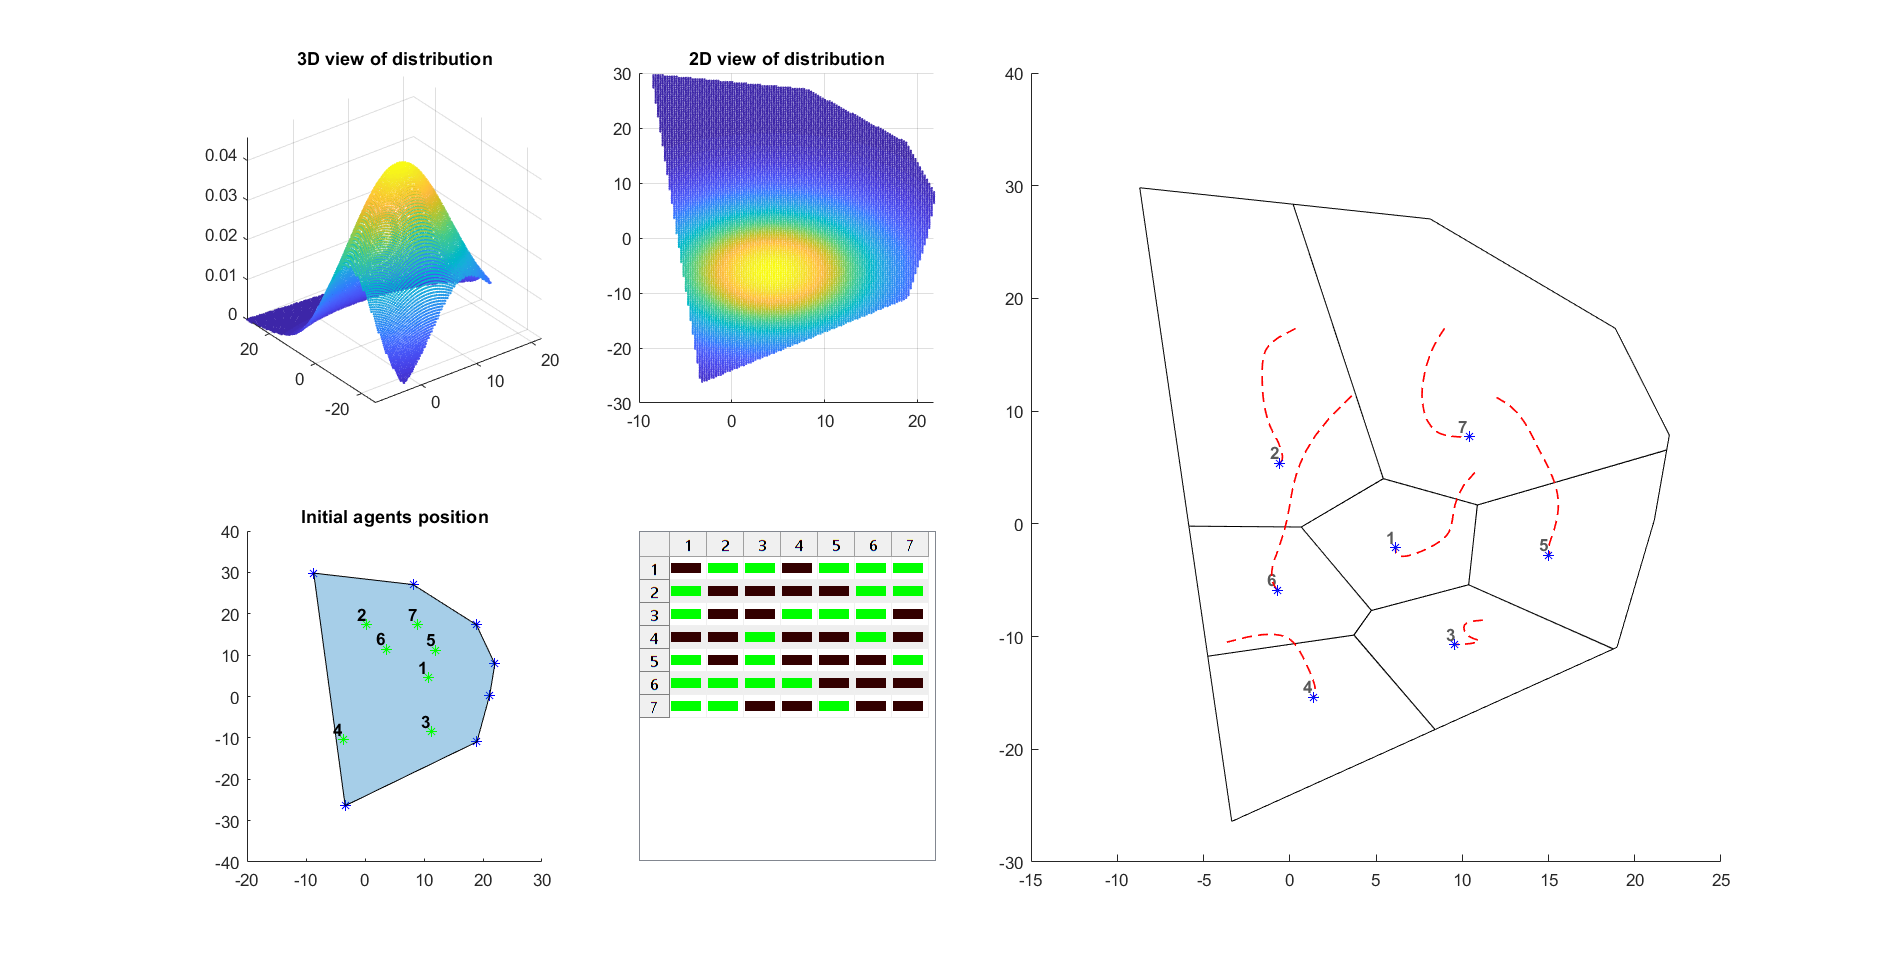
\includegraphics[scale=0.45,angle=90]{figs/convergenceResultsA.png}
		\caption{Results with 7 agents (ver. A)}\label{fig:convergenceResultsA.png}	
	\end{figure}
	
	\begin{figure}	
		\centering	
		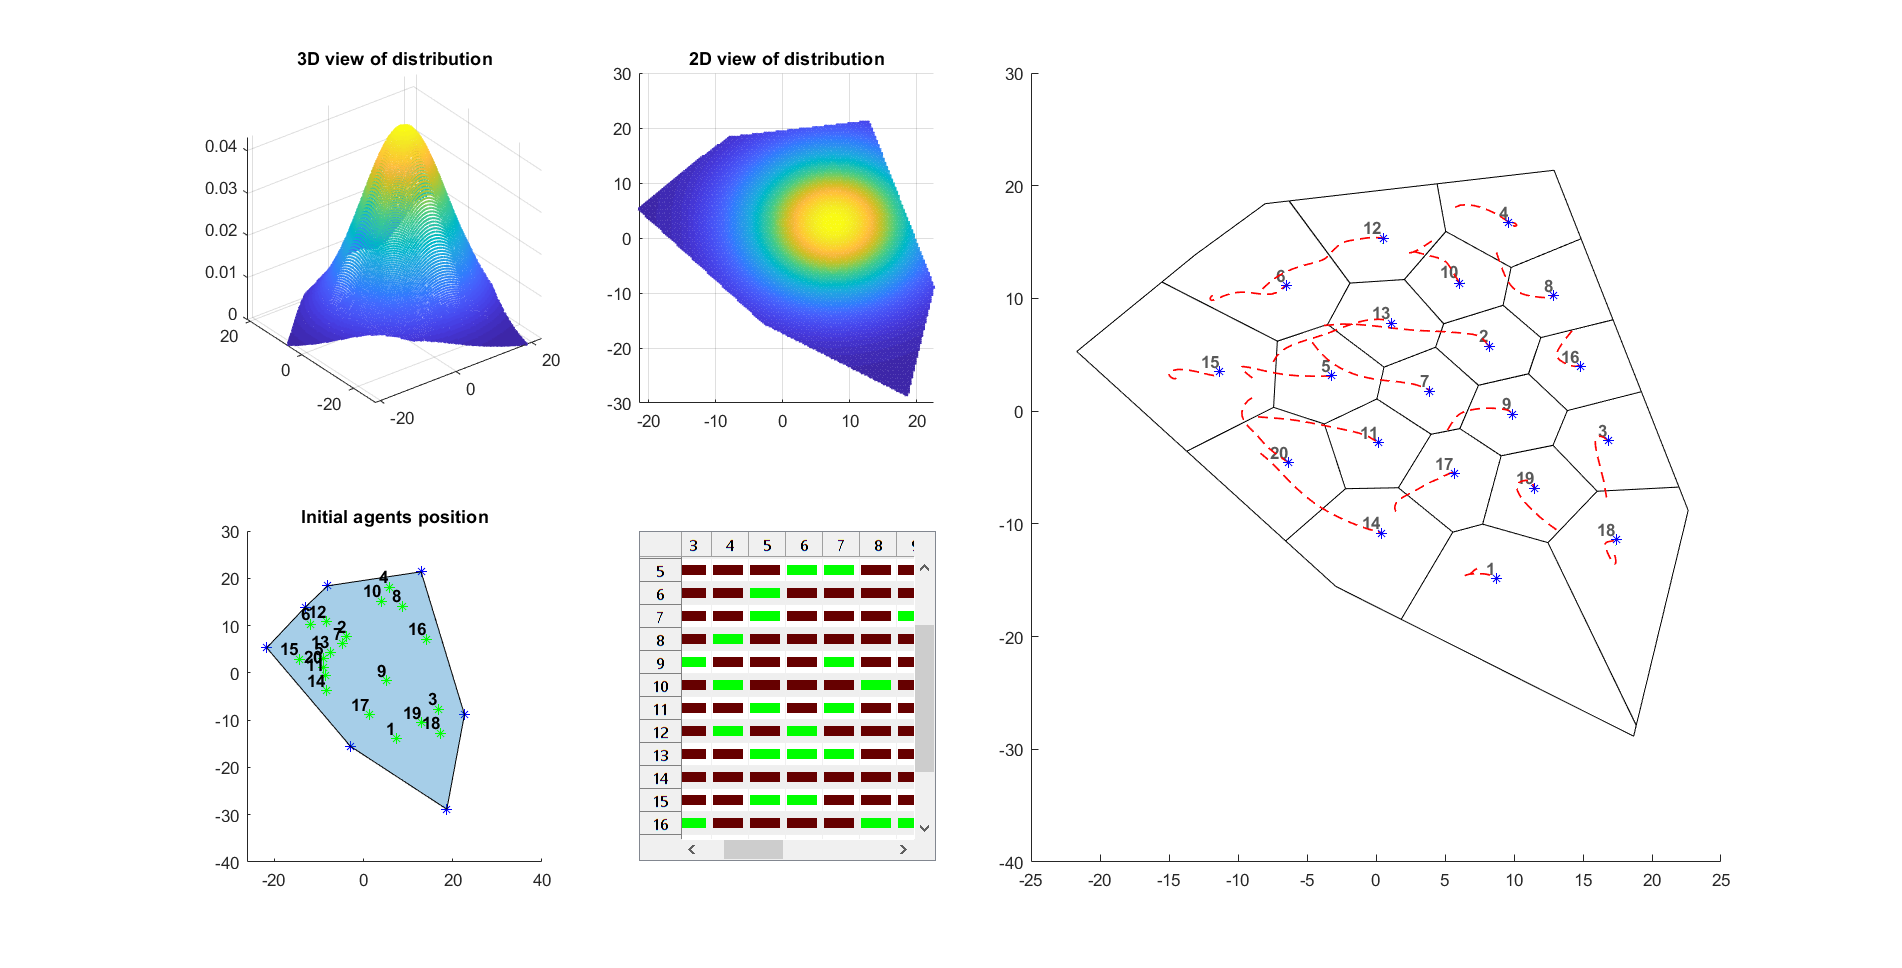
\includegraphics[scale=0.45, angle=90]{figs/20convergenceResultsA.png}
		\caption{Results with 20 agents (ver. A)}\label{fig:20convergenceResultsA.png}	
	\end{figure}
	
	\section{Online algorithm (B)}
	This algorithm is not much slower than the first version, especially for few agents.\\
	It may be faster if implemented with a better communication between agents (instead of r/w files), but not by a large margin.\\
	
	It is of interest to see how they both arrive to similar results but not exactly the same; this is due to the fact that while in the offline algorithm every agent "sense" the others between deciding the next control step, thus continuously updating the centroid.\\
	In the distributed version, the centroid is updated only when the agent reaches it, making the trajectories of the centroids (and thus of the agents) slightly different.
	
	\begin{figure}	
		\centering	
		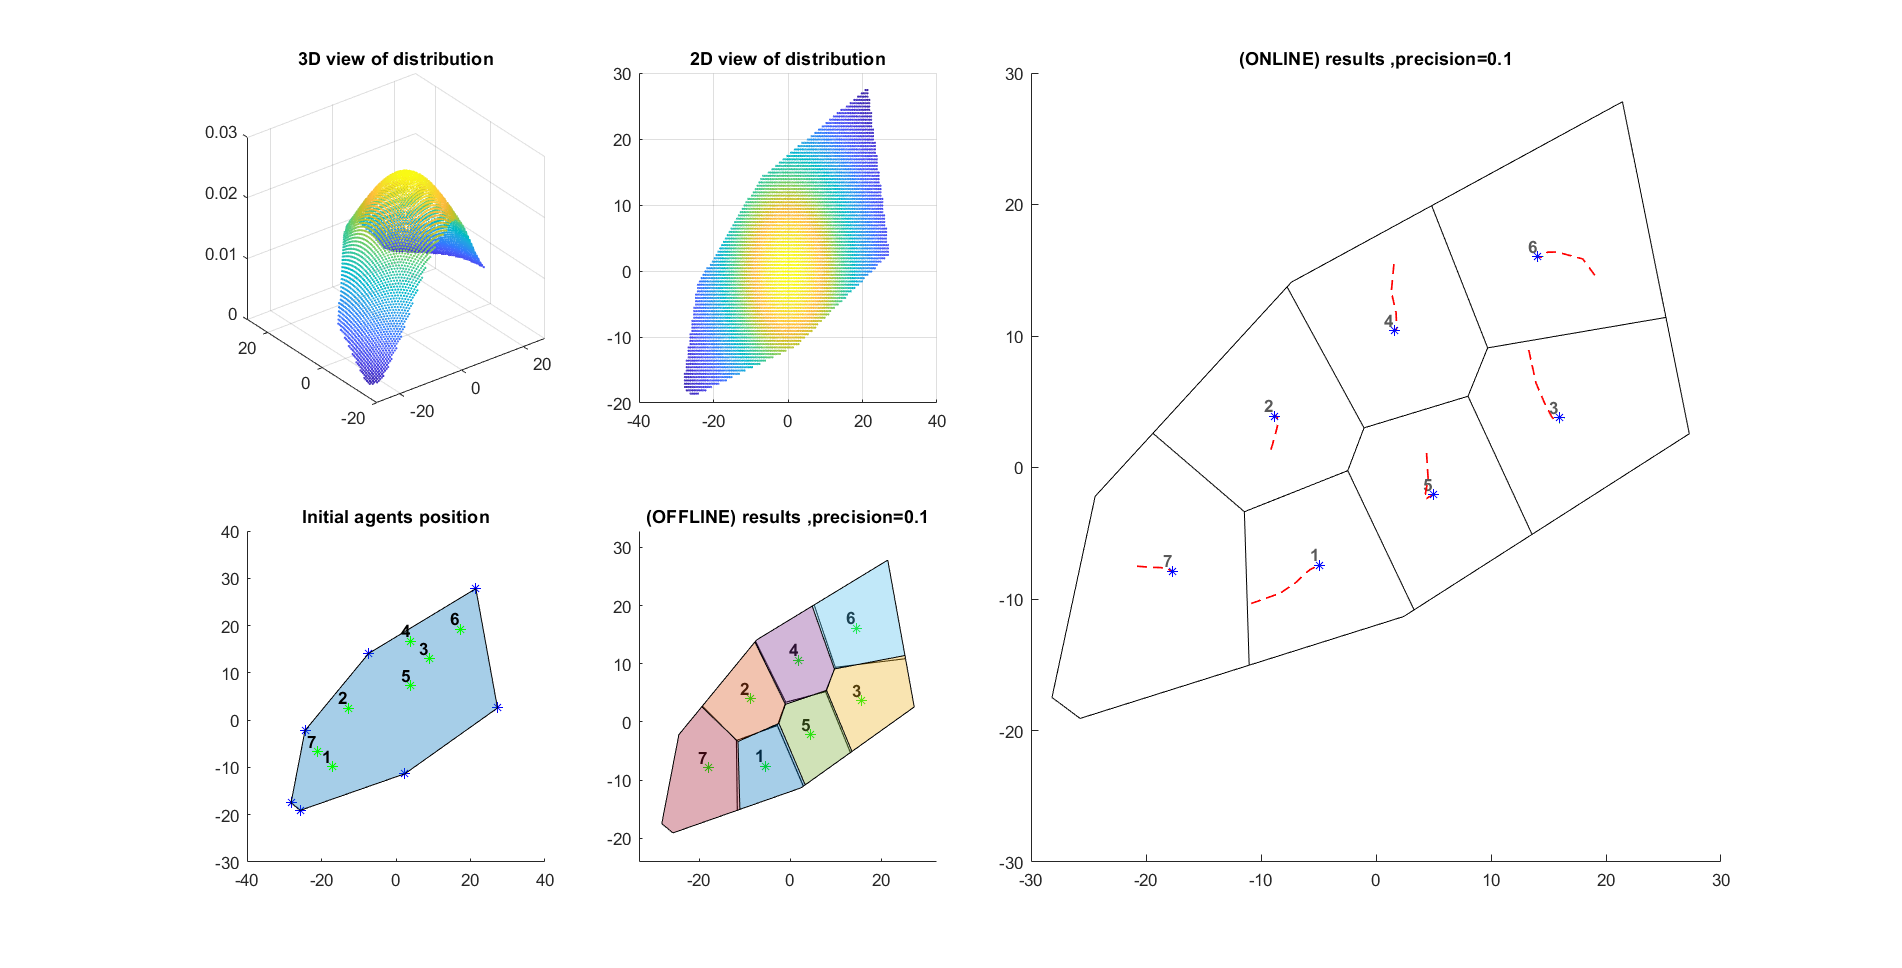
\includegraphics[scale=0.45,angle=90]{figs/convergenceResultsB.png}
		\caption{Results with 7 agents (ver. B)}\label{fig:convergenceResultsB.png}	
	\end{figure}
	
	\begin{figure}	
		\centering	
		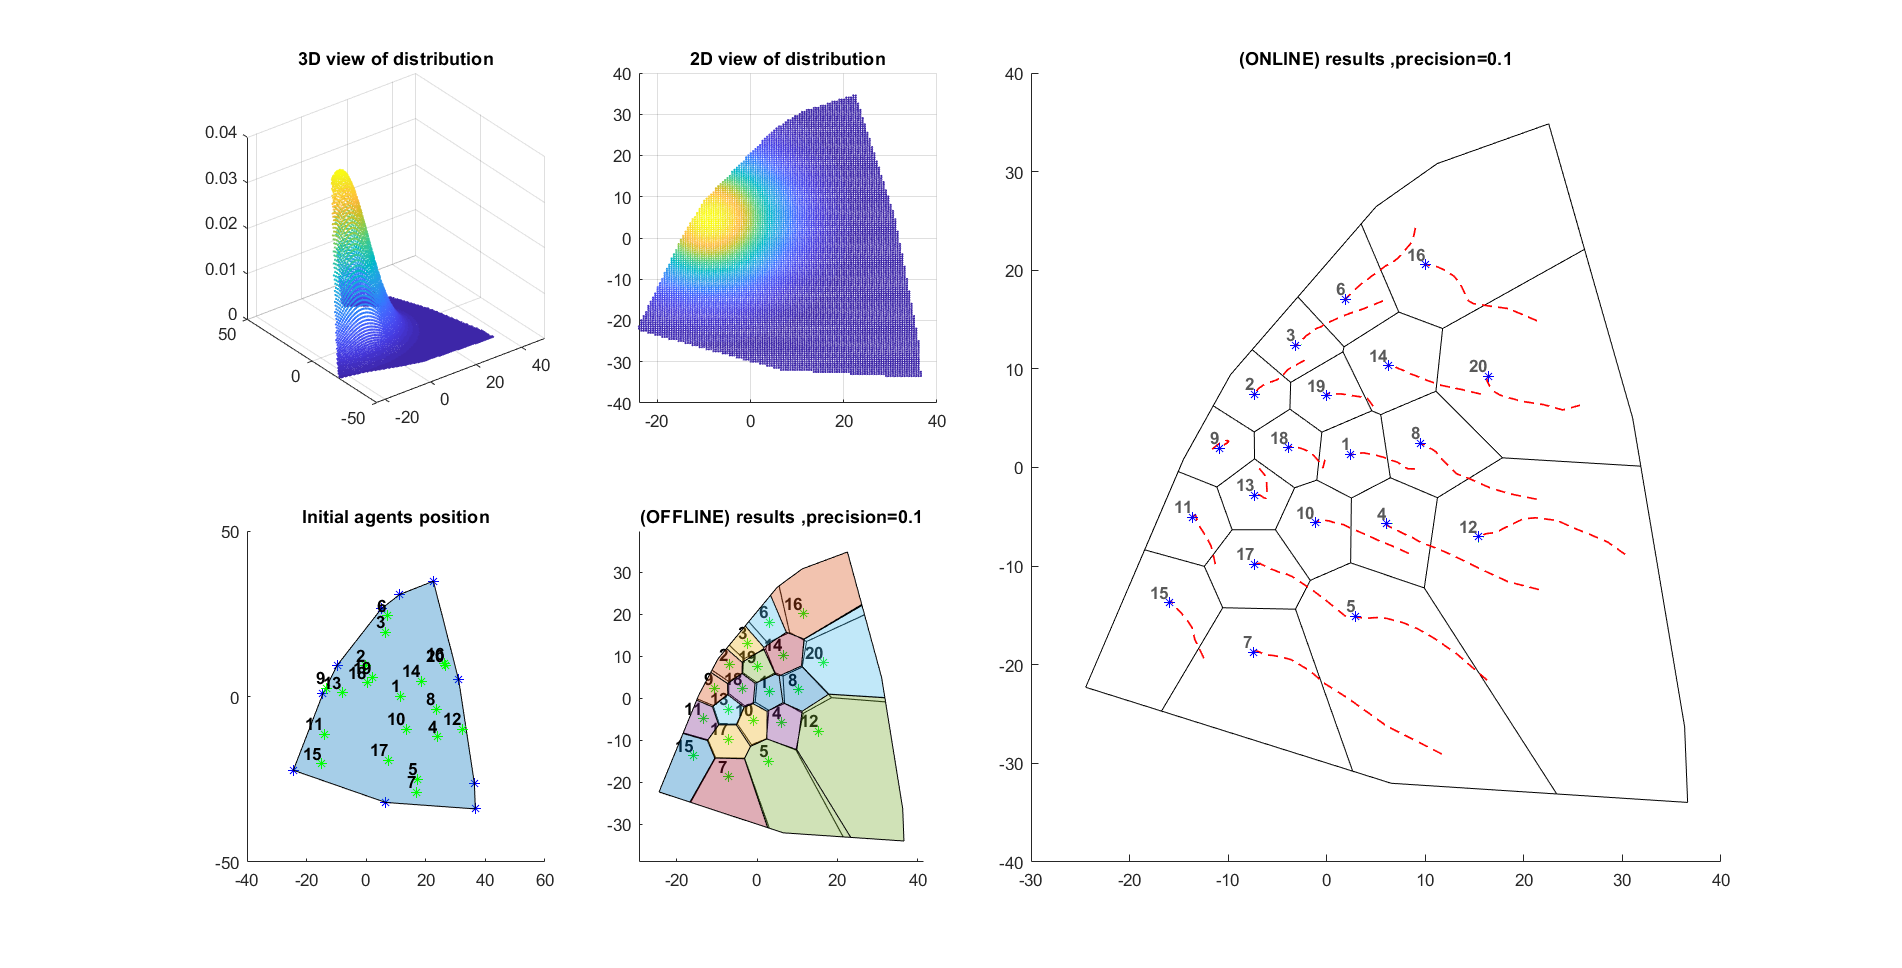
\includegraphics[scale=0.45, angle=90]{figs/20convergenceResultsB.png}
		\caption{Results with 20 agents (ver. B)}\label{fig:20convergenceResultsB.png}	
	\end{figure}
	
	
	%%%%%%%%%%%%%%%%%%%%%%%%%%%%%%%%%%%%%
	
	%%%%% SVILUPPI FUTURI %%%%%%
	\chapter*{Conclusions} % and future developments}
	\addcontentsline{toc}{chapter}{Conclusions} %  and future developments}
	%%%%%%%%%%%%%%%%%%%%%%%%%%
	The obtained results seem to be consistent with those to be expected from the main research paper, made exception for the timing and event control; we think that this work may be a good starting step to realize a real Coverage Control for Cooperative Multi-Robot Networks.\\\\
	
	Some code optimization issues have been neglected from the efficiency point of view, nonetheless the execution times are kept reasonably short.\\
	We believe that the next logical step would be to fix this aforementioned speed issues, by e.g. finding a more efficient Voronoi cell computation, and to implement the timing and scheduling of different control parts on real platforms, which would be way easier and of more significance than only the simulation.
	
	% %%%% APPENDIX %%%%%
	% \appendix
	% \chapter{Appendix title}
	% %%%%%%%%%%%%%%%%%%%%
	
	%%%%%%%%%% BIBLIOGRAPHY %%%%%%%%%%%%%%
	\begin{thebibliography}{9}             %crea l'ambiente bibliografia
		
		%%%%%%%%%%%%%%%
		
		\addcontentsline{toc}{chapter}{Bibliography}
		
		\bibitem{K1} J. Cortes, S. Martinez, T. Karatas, F. Bullo. "Coverage Control for Mobile Sensing Networks"
		IEEE Transactions on Robotics and Automation, Vol. 20, No. 2, April 2004
		\bibitem{K2} T. Hayes and F.H. Ali. "Mobile Wireless Sensor Networks: Applications and Routing Protocols" Handbook of Research on Next Generation Mobile Communications Systems. 2016.
		%%%%%%%%%%%%%%%%%%%%%%%%%%%%%%%%%%%%%%
		
	\end{thebibliography}
	
	
\end{document}